\documentclass[aps,pre,twocolumn,showpacs,amsmath,amssymb]{revtex4-1}
\usepackage{graphicx}
\usepackage{color}
\usepackage[portuguese]{babel}
\usepackage[utf8]{inputenc}
\usepackage[T1]{fontenc}
\usepackage[shortlabels]{enumitem}
\hfuzz 1pt
\vfuzz 1pt
\setlength{\parskip}{\baselineskip}

\begin{document}

\title{Exercício 06: Integração Numérica}

\author{Ernesto González*, Iara Tiago*, Ariana Dias*}

\begin{abstract}
 Integração numérica de funções contínuas com a regra do trapézio, de Simpson e método de Romberg. Exemplo do trabalho da impulsão da esfera. Integração numérica em conjuntos discretos de dados com a regra do trapézio e de Simpson. Exemplo de velocidade de saída de uma flecha.
\end{abstract}

\maketitle

\section{Esfera Imersa em Água}
Considere-se uma esfera de 2 metros de raio, parcialmente imergida em água. Sabe-se que o volume da esfera fora da água é $V=\dfrac{\pi}{3}h^2(3r-h)$, em que $h$ é a altura da secção fora de água. Pretende-se calcular o trabalho realizado pela impulsão durante o processo de submergir metade da esfera.\\
Utilizaram-se a regra do trapézio, de Simpson e método de Romberg para calcular numericamente o trabalho realizado pela impulsão.
Pelo princípio de Arquimedes, a impulsão, $I$, é obtida através da equação $I=\rho Vg$, sendo
$\rho=10^3$Kg/m$^3$ e $g=9.8$m/s$^2$. Como $r=2$, o volume é dado por $V=\dfrac{\pi}{3}h^2(6-h)$. Inicialmente, com a esfera fora de água a altura da secção fora de água é o diâmetro da esfera, $h=4$. Após submergir metade da esfera, a altura da secção fora de água é $h=2$.

Assim, o trabalho realizado pela impulsão é dado por
\begin{equation}
    \int_2^4 Fdr=\int_2^4 I(h)dh=\int_2^4 \rho \dfrac{\pi}{3}h^2(6-h)g dh
\end{equation}

De forma a verificar os valores obtidos do cálculo deste trabalho com os métodos mencionados, foi utilizada a função Integrate do \textit{Mathematica}.

\begin{table}[hbt!]
\centering
\caption{Valores do trabalho W, obtidos em cada método de integração e no \textit{Wolfram Mathematica}, com uma precisão de $10^-^2^0$ e $n$ correspondente ao número de divisões de W, para que este consiga convergir para um determinado valor.}
\begin{tabular}{|c|c|c|c|}
    \hline
n & Método & Valor de W       \\ \hline
100 & Trapézio & 123150.76  \\ \hline
100 & Simpson & 123150.43  \\ \hline
- & Romberg & 128284.19  \\ \hline
- & \textit{NIntegrate} & 123150.43  \\ \hline
\end{tabular}
\end{table}

\section*{Alínea b}

\begin{figure}[h!]
   \begin{center}
    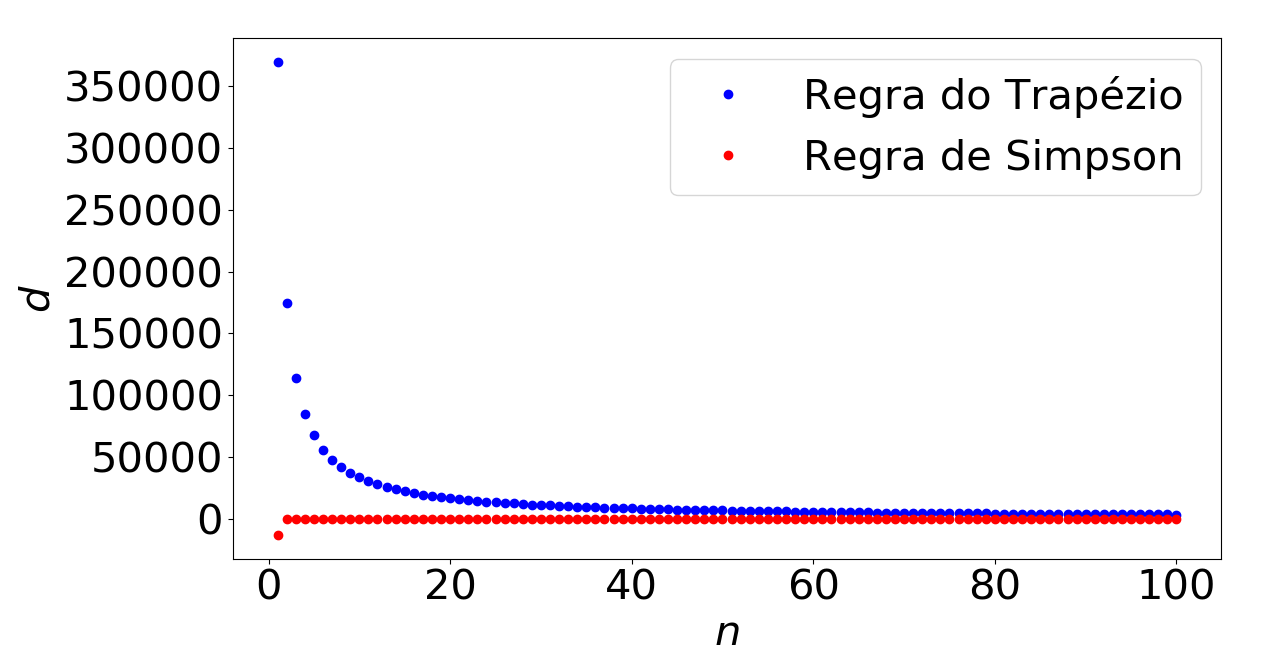
\includegraphics[width=\columnwidth]{desviointegralporiter.png} \\
\caption{Gráfico que relaciona o desvio do integral obtido com a regra do trapézio e o método de Simpson, em função do número de divisões de integração.}
  \label{fig.exemplo}
   \end{center}
  \end{figure}


O método de Simpson só funciona corretamente, perante uma boa escolha do número de divisões de integração, $n$. Este método, aproxima a função com que trabalha, por meio de segmentos de parábolas, que são obtidas por polinómios de segundo grau. Como tal, para a regra de Simpson, deve ser escolhido um $n$ par.
Por outro lado, a regra trapézio leva mais tempo a convergir, sendo necessário um maior número de divisões de integração para que se observe a sua curva a aproximar-se de um valor específico.
Pela Figura 1 consegue-se, assim, observar e confirmar, que o método de Simpson é mais eficaz que a regra do trapézio, o que também pode ser confirmado pela Tabela I, uma vez que a regra do trapézio em \textit{Python} e a função NIntegrate do \textit{Mathematica} dão o mesmo resultado.\\

Para o método de Romberg fez-se um gráfico do erro do método em função do número de iterações, $k$, (em escala log-lin) como na Figura 2. Observa-se que o erro decai rapidamente, em apenas 19 iterações, para uma precisão de $\epsilon=10^{-16}$, para um valor de $0.0$. Para a primeira iteração, $k=1$, o valor do integral corresponde a $-123150.432021$. Este valor é igual ao valor do cálculo do integral pela regra de Simpson.
Face à rapidez de diminuição do erro associado ao método opta-se por representar este numa escala logaritmica para a melhor compreensão do processo possível.

\begin{figure}[h!]
   \begin{center}
    \includegraphics[width=\columnwidth]{Romberg.png} \\
\caption{Gráfico do logaritmo do erro associado ao Método de Romberg, $\epsilon_s$ em função do número de iterações, $k$. Pode-se observar que o erro diminui rapidamente, ao final de 19 iterações para 0.0.}
  \label{fig.exemplo}
   \end{center}
  \end{figure}

\section{Integral do inverso do quadrado}
Considere-se a função $f(x)=\frac{1}{x^2}$. Pretende-se calcular o integral de $f$ em, por exemplo, $x\in[0.1,5,1]$. Resolvendo analiticamente, vem\\
\begin{equation}
    \int_{0.1}^{50.1}f(x)=\left[-\frac{1}{x}\right]^{50.1}_{0.1}=-\frac{1}{50.1}+10 \approx 9.98003992
\end{equation}
Calculemos agora o valor do integral usando a regra do trapézio, a regra de Simpson e o método de Romberg. Na Figura 3 encontra-se o valor do desvio $d=I_{numérico}-I_{real}$ em função do do tamanho da divisão usada no método numérico, em que $I_{numérico}$ é o valor do integral obtido numericamente e $I_{real}=9.98003992$.\\
\begin{figure}[hbt!]
  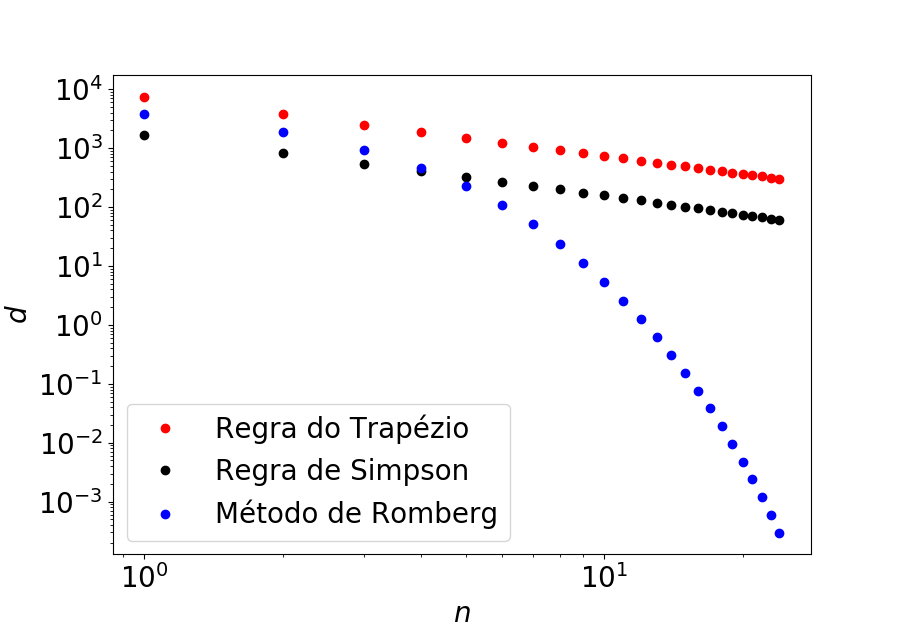
\includegraphics[width=\columnwidth]{desvioinversesquare.png}
  \caption{Desvio, $d=I_{real}-I_{numerico}$, do resultado do integral calculado numericamente ao valor real do integral, pela regra do trapézio, regra de Simpson e método de Romberg, em função do número de divisões, $n$. O método de Romberg foi aplicado com número de iterações máximo $k_{max}=25$ e critério de convergência $\epsilon=10^{-6}$.}
  \label{desvioinversequare}
\end{figure}

\section{Arco e flecha}
A força, $F(x)$, necessária para esticar o fio de um arco é apresentada na Tabela II.\\
\begin{table}[hbt!]
\caption{Valor da força $F(x)$ necessária para esticar o fio do arco para um afastamento $x$.}
\begin{tabular}{|c||c|c|c|c|c|c|}
    \hline
x(m) & 0.00 & 0.05 & 0.10 & 0.15 & 0.20 & 0.25 \\ \hline
F(N) & 0 & 37 & 71 & 104 & 134 & 161 \\ \hline \hline
x(m) & 0.30 & 0.35 & 0.40 & 0.45 & 0.50 & \\ \hline
F(N) & 185 & 207 & 225 & 239 & 250 &  \\ \hline
\end{tabular}
\end{table}
A velocidade de saída de uma flecha de $m=0.00075\,kg$ quando o fio é esticado $0.5\,m$ é dada por
\begin{equation}
\begin{split}
    W = \Delta E_c  \iff &\int_{0.00}^{0.50}F(x)dx = \frac{m v^2}{2}
    \\
    \iff &v=\sqrt{2\int_{0.00}^{0.50}\frac{F(x)}{m}\,dx}
\end{split}
\end{equation}
Recorreu-se, assim, ao método do trapézio, adaptado a conjuntos discretos, para o cálculo do integral a partir de uma lista de dados como na Tabela II. Obteve-se $F = 74.4 N$  para o valor do integral e uma velocidade de saída $v = 44.54211 ms^{-1}$.\par
De seguida, recorreu-se à função Interpolation para ordem 1 do \textit{Mathematica} e fez-se o gráfico da função interpolada, como se pode verificar na Figura 4.
\begin{figure}[hbt!]
   \begin{center}
    \includegraphics[width=\columnwidth]{Interpolation.png} \\
\caption{Gráfico resultante da função \textbf{Interpolation} para ordem 1 do \textit{Mathematica} em relação à função $F(x)$ em relação à distância,$x$. $F$ varia entre $0$ e $250$ e $x$ entre $0.00$ e $0.50$}
   \end{center}
  \end{figure}

Recorreu-se ainda a função NIntegrate do \textit{Mathematica} para o resultado obtido para a interpolação anteriormente calculada no intervalo $x = [0,0.5]$ obtendo-se um valor de $F = 74.4 \,N$.
Pode-se verificar que ambos os valores obtidos por recurso ao método do Trapézio como ao NIntegrate do \textit{Mathematica} são iguais, que pode ser justificado pelo facto de o \textit{Mathematica} por \textit{default} recorrer a um método muito similar ao método do trapézio para o cálculo do integral. O motivo pelo qual se optou por uma interpolação de ordem 1 no \textit{Mathematica} deve-se ao desconhecimento da dependência de $F$ sobre $x$ pelo que, primeiramente, se considera a aproximação linear.\\
De seguida pretendeu-se calcular $W_{0.00\rightarrow0.50}$ pela regra de Simpson. Para tal foram seguidos três procedimentos diferentes:\\
\begin{enumerate}[a)]
    \item usou-se a função scipy.interpolate.interp1d para interpolar os dados, obtendo-se uma função interpolada de terceira ordem e, de seguida, aplicou-se a regra de Simpson para funções contínuas;\\
    \item usou-se o método Interpolate[] e depois aplicou-se Series[] para obter o desenvolvimento de Taylor de ordem 3 em $x=0.25$ da função interpolada pelo \textit{Mathematica} e aplicou-se a regra de Simpson para funções contínuas; \\
    \item usou-se a regra de Simpson para conjuntos discretos de dados.
\end{enumerate}
Na Tabela III encontram-se os resultados obtidos para os diferentes procedimentos.
\begin{table}[hbt!]
\centering
\caption{Cálculo do integral pela regra de Simpson e respetiva velocidade de saída associada por três procedimentos: interpolação dos dados com scipy para um polinómio de grau 3 e aplicação da regra de Simpson; interpolação dos dados com Interpolate[] e aplicação da regra de Simpson ao desenvolvimento de Taylor de ordem 3 em $x=0.25$ obtido pelo Series[]; aplicação da regra de Simpson para conjuntos discretos de dados.}
\begin{tabular}{|c|c|c|} \hline
\text{Procedimento} & $W_{0.00\rightarrow0.50}$ & $v$ \\ \hline
scipy.interpolate.interp1d & 74.523840 & 44.579170 \\ \hline
Series[Interpolate[]] & 74.750000 & 44.646762 \\ \hline
Simpson Discreto & 74.533333 & 44.582009 \\ \hline
\end{tabular}
\end{table}

\end{document}
